\chapter{Методика атомно-зондовая томография}\label{ch:ch1}

В основе атомно-зондовой томографии(АЗТ) лежат три основных принципа. Один принцип - возможность испарения материала с помощью постоянного электрического поля (в некоторых случаях с импульсной составляющей). Второй - времяпролетная масс-спектрометрия. Третий - проекционный принцип восстановления трехмерного взаиморасположения атомов. Какие-ото общие слова про томограф (составляющие, потатомное испарение)

\section{Полевое испарение в атомно-зондовой томографии}\label{sec:ch1/sec1}

\nomenclature{\(АЗТ\)}{атомно-зондовая томография}
В атомно-зондовой томографии используется принцип полевого испарения для того, чтобы последовательно удалять атомы от поверхности образца. Испарение происходит путем ионизации атомов с поверхности образца с последующим ускорением в электрическом поле. Ионизация происходит из-за комбинации воздействий постоянного напряжения и высоковольтного или лазерного импульса, приложенного к поверхности образца. Первой методикой, использовавшей данные механизмы, была полевая ионная микроскопия \cite{Muller60}. В последствии атомно-зондовая томография заимствовала часть методов из автоионной микроскопии.
В настоящий момент механизм испарения отдельных атомов с помощью электрического поля не описан достаточно полно и точно. Обычно, для объяснения данного механизма используются простые термодинамические соображения. Одно из первых описаний испарения с помощью электрического поля представил Миллер \cite{Muller56}. Контролируемое испарение атома представлялось как прохождение атомом энергетического барьера на поверхности образца. В модели Мюллера считается, что испаренный атом имеет такую же энергию, как атом, абсорбированный на поверхности образца. В случае отсутствия приложенного к образцу поля, энергия $Q_0$, необходимая для удаления атома от поверхности и его n-кратной ионизации, может быть оценена с помощью цикла Борна-Габера.

\begin{equation}
	\label{eq:equation1}
	Q_0 = \Lambda + \sum_{1}^{n} I_i -n\phi_e
\end{equation}

где $\Lambda$ - энергия сублимации, $I_i$ - энергия ионизации, $\phi_e$ - работа выхода электрона, n - количество электронов. Значения энергий ионизации, сублимации и работа выхода электрона известны дя атомов большинства сортов и могут считаться табличными. Ниже представлены графики для энергетического барьера атома на поверхности образца.

\begin{figure}[ht]
	\begin{minipage}[b][][b]{0.49\textwidth}\centering
		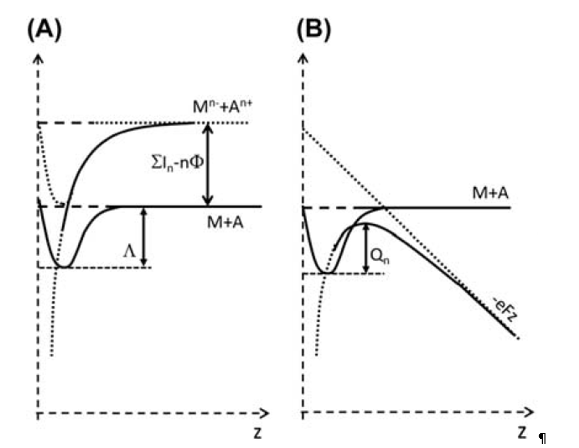
\includegraphics[width=\textwidth]{mullerenergy} \\ а)
	\end{minipage}
	%\hfill
	\begin{minipage}[b][][b]{0.49\textwidth}\centering
		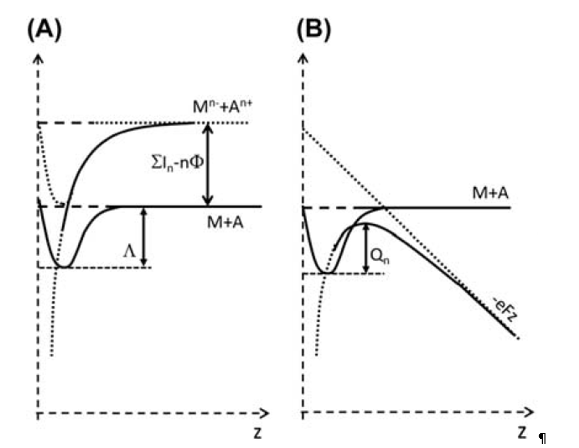
\includegraphics[width=\textwidth]{mullerenergy} \\ б)
	\end{minipage}
	\caption{Диаграмма потенциальной энергии атома без приложенного электрического поля (а), с приложенным электрическим полем (б)}
	\label{fig:mulener}
\end{figure}

Приложив внешнее электрическое поле к образцу, можно снизить потенциальный барьер, необходимый для испарения атома. Высота барьера Q(F) может быть описана следующей формулой \cite{Muller56}:

\begin{equation}
	\label{eq:equation2}
	Q(F) = Q_0 - \sqrt{\frac{n^3 e^3}{4\pi\epsilon_0}F}
\end{equation}

где $\epsilon_0$ - диэлектрическая проницаемость в вакууме, F - напряженность поля. Слагаемыми второго порядка, отвечающими поляризации атомов поверхности, как правило, пренебрегают. Поскольку основной задачей АЗТ является контролируемое по-атомное испарение, то необходимо контролировать скорость испарения атомов. Вероятность испарения может считаться термически активированным процессом, соответственно она может быть описана законом Аррениуса:

\begin{equation}
	\label{eq:equation3}
	P_{evap} \propto \exp(-\frac{Q(F)}{k_B T})
\end{equation}

где Q(F) - высота энергетического барьера \cref{eq:equation2}, $k_B$ - постоянная Больцмана, T - температура образца в Кельвинах. Скорость испарения определяется как:

\begin{equation}
	\label{eq:equation4}
	\Phi_{evap} = \nu_0\exp(-\frac{Q(F)}{k_B T})
\end{equation}

где $\nu_0$ - характерная частота колебаний атомов в направлении по нормали к поверхности образца. Данная зависимость подтверждена экспериментально \cite{Kellogg81,Kellogg84}, на Рисунке \cref{fig:evapspeed} представлены экспериментальные зависимости скорости испарения от приложенного электрического поля (в относительных величинах). Также наблюдались отклонения от данной зависимости \cite{Gomer84,Wada84}, которые характерны для температур менее 40 К и для ионов малой массы.

\begin{figure}[ht]
	\centerfloat{
		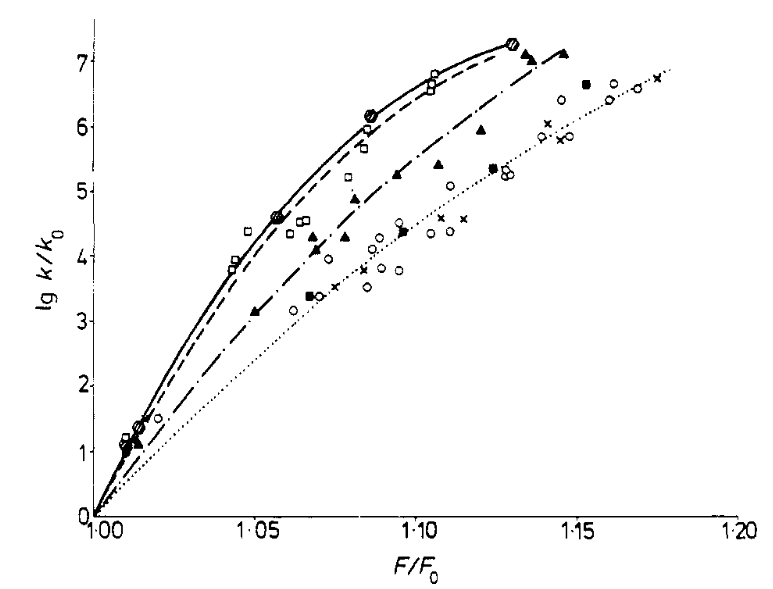
\includegraphics[scale=0.8]{evapspeed}
	}
	\caption{Зависимость скорости испарения от приложенного электрического поля для различных металлов в относительных единицах\cite{Tsong78}}
	\label{fig:evapspeed}
\end{figure} 

Значение поля, при котором величина энергетического барьера снижается до нуля, как правило, называется полем испарения $F_{evap}$. Учитывая \cref{eq:equation1} и \cref{eq:equation2}, это поле может быть вычислено для различных зарядовых состояний с помощью следующей формулы: 

\begin{equation}
	\label{eq:equation5}
	\Phi_{evap} = \frac{4\pi\epsilon_0}{n^3 e^3}(\Lambda + \sum_{1}^{n} I_n - n\phi_e)^2
\end{equation}

Результаты расчетов поля испарения для различных зарядностей ионов, на основе этого выражения, могут значительно различаться. Например, поле испарения для вольфрама принимает значения 102, 57, 52 и 62 В/нм для зарядностей +1, +2, +3 и +4, соответственно. Значения поля испарения для большинства элементов для наиболее распространенных зарядностей можно найти в справочной литературе. В работе Брандона \cite{Brandon65} было сделано предположение о том, что поле испарения определяется наименьшим из значений полей испарения для разных зарядностей иона. Данное предположение нашло хорошее подтверждение в проведенных экспериментах \cite{Tsong782}. Для большинства металлов поле испарения лежит в диапазон от 10 до 60 В/нм.
Поскольку на полевое испарение оказывает влияние температура и приложенное поле, то существует теоретически бесконечное число сочетаний значений поля и температуры, отвечающие одной и той же скорости испарения. В первом приближении высоту энергетического барьера рассматривают как величину, линейно меняющуюся весте с линейным изменением поля:
 
\begin{equation}
	\label{eq:equation6}
	Q(F) = Q_0(1 - \sqrt{1 - \sqrt{\frac{F}{F_{evap}}}}) \approx Q_0 (1 - \frac{F}{F_{evap}})
\end{equation}

Используя данное упрощенное выражение вместе с формулой \cref{eq:equation4} можно получить зависимость электрического поля необходимого для поддержания определенной скорости испарения в зависимости от температуры:

\begin{equation}
	\label{eq:equation7}
	\frac{F}{F_{evap}} \approx 1 + \ln{\frac{\Phi_{evap}}{\nu_0}\frac{k_B T}{Q_0}}
\end{equation}

Это простое выражение хорошо согласуется с экспериментальными наблюдениями различных авторов \cite{Kellogg84,Kellogg81,Wada84,Kellogg80,Vurpillot06}. Оно проиллюстрировано на Рисунке  \cref{fig:field_temp}, где поле, необходимое для испарения образца из чистого вольфрама регистрировалось как функция температуры. Соответствующее фактическое значение поля для заданной температуры обычно называют эффективным полем испарения.

\begin{figure}[tb]
	\centerfloat{
		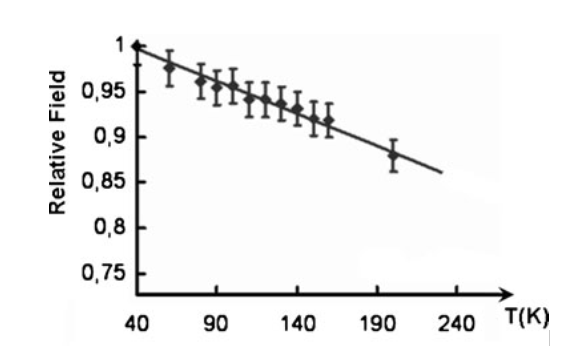
\includegraphics[scale=0.8]{field_temp}
	}
	\caption{Зависимость поля от температуры при постоянной скорости детектирования \cite{Vurpillot06}}
	\label{fig:field_temp}
\end{figure} 

\FloatBarrier


Как правило, такие кривые (как на Рисунке \cref{fig:field_temp}) используются для калибровки параметров сбора данных, то есть определения оптимальной температуры, скорости испарения и т.д. Вада, измеряя такие калибровочные кривые для чистых металлов, подчеркнул, что разные элементы будут иметь разные кривые \cite{Wada84}. При этом в сплавах будет иметь место сложная комбинация полей испарения каждого элемента в зависимости от химического состава и типов связей между элементами.

\FloatBarrier

\section{Времяпролетная масс-спектрометрия в атомно-зондовой томографии}\label{sec:ch1/sec2}

Начиная с  1967 года, когда был собран первый атомно-зондовый томограф Мюллером, Паницем и МакЛайном в Государственном университете Пенсильвании \cite{Muller68} времяпролетная масс-спектрометрия была неотъемлемой частью атомно-зондовых томографов. Простые предположения и уравнения, предложенные в то время, до сих пор регулярно используются в современных установках АЗТ для определения химической природы испаряемых ионов. Конечные результаты, такие как состав и трехмерные координаты атомов, зависят от качества обработки масс-спектра.
Качество масс-спектра зависит не только от физики полевого испарения, но и от конструкции АЗТ, условий сбора данных, характера обработки данных. В АЗТ атомы испаряются с помощью электрического поля, они ионизируются и ускоряются в электрическом поле, окружающем поверхность образца (см. общие принципы работы в разделе \cref{sec:ch1/sec4}). Некоторые из этих ионов собираются детектором, используемым для определения времени и места удара. Время полета иона – это время, необходимое для полета от поверхности образца до детектора, которое называется длиной полета L (см. Рисунок \cref{fig:time_flight}). 

\begin{figure}[htb]
	\centerfloat{
		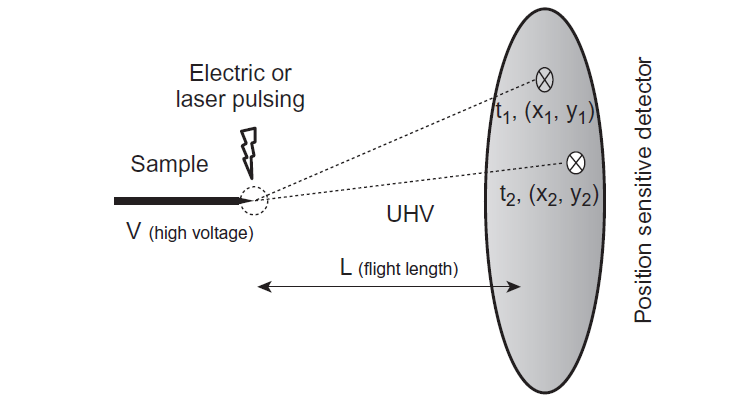
\includegraphics[scale=0.8]{time_flight}
	}
	\caption{Схема измерения времени пролета иона в АЗТ}
	\label{fig:time_flight}
\end{figure} 

Время пролета можно измерить только в том случае, если испарение инициируется напряжением или лазерным импульсом. Тогда, если предположить, что ионы не имеют начальной скорости и имеют постоянную скорость во время полета и что вся их энергия превращается в кинетическую энергию, то отношение массы к заряду M ионов записывается как:

\begin{equation}
	\label{eq:equation8}
	M = \frac{m}{n} = 2eV(\frac{t_f}{L})^2 = kV(\frac{t_f}{L})^2
\end{equation}

где m — масса иона, n — заряд, V — полное напряжение, приложенное к образцу, e — элементарный заряд электрона, L — длина полета и $t_f$ — время полета. Масса иона выражается в относительных единицах массы (а.е.м.). В современных установках АЗТ типичная длина полета составляет от 10 до 50 см, что дает характерное время полета в диапазоне около 1–5 мкс при напряжении в диапазоне 1–10 кВ.
Масс-спектр представляет собой гистограмму, высота каждого столбца гистограммы равна числу ионов задтектированных в соответствующем диапазоне масс. Как показано на Рисунке \cref{fig:mass_spectr}, на масс-спектре возможно присутствие пики, соответствующие ионам разной зарядности.

\begin{figure}[ht]
	\centerfloat{
		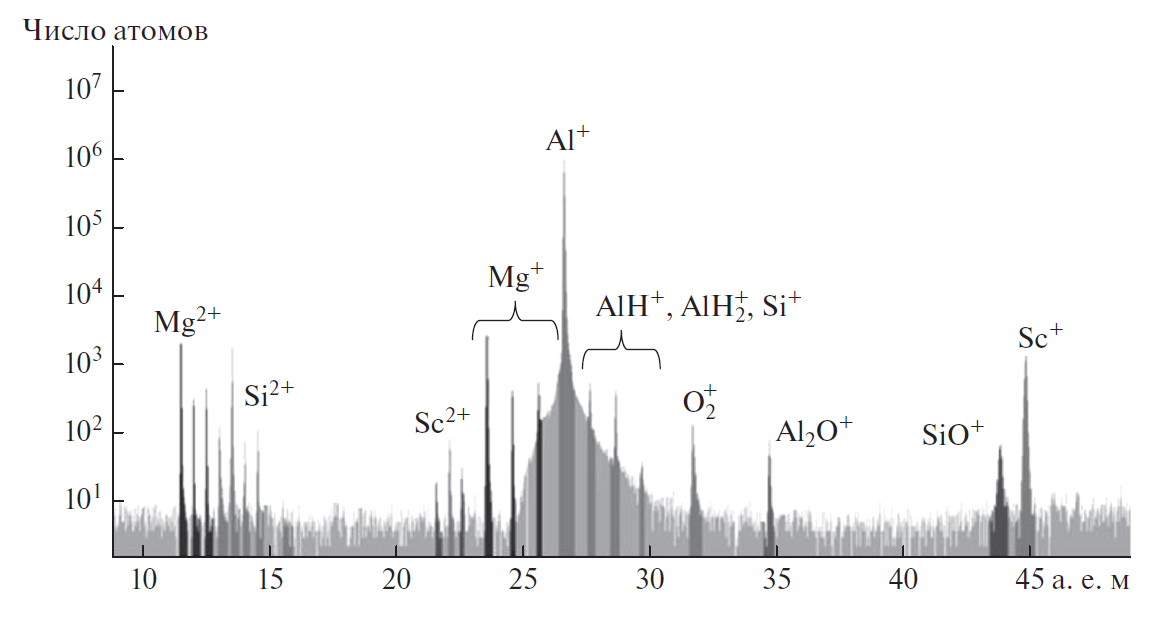
\includegraphics[width=\textwidth]{mass_spectr}
	}
	\caption{Пример масс-спектра атомно-зондовых данных, полученный в работе \cite{scbibAlumYAFI}}
	\label{fig:mass_spectr}
\end{figure} 

Идентификация пиков в масс-спектрах зависит как от предварительного знания химии анализируемого материала, так и от естественного содержания изотопов. Например, на Рисунке \cref{fig:mass_spectr} идентифицированы различные изотопы Mg$^{2+}$ (выделены в левой части спектра черным цветом). Стоит отметить, что одной из особенностей метода АЗТ является необходимость уточнения параметров восстановления масс-спектра для каждого эксперимента. Качество масс-спектра оценивают по разрешению по массе $\frac{M}{\Delta M_x}$, где $\Delta M_x$ — ширина пика масс-спектра на определенной высоте от максимальной высоты пика. Разрешение по массе обычно измеряется на уровне 50 $\%$ (полная ширина на половине высоты, FWHM), также возможны оценки на 10 $\%$ и 1 $\%$ от максимума пика. Разрешение по массе зависит от геометрических факторов (длина и траектория полета) и точности измерений (времени пролета и напряжения). Оптимизация разрешения по массе может осуществляться с помощью аппаратного обеспечения (например, рефлектронов) или применения специальных алгоритмов оптимизации при обработке данных \cite{Shutov19}.

\FloatBarrier

\section{Проекционный принцип восстановления координат атомов}\label{sec:ch1/sec3}

Как уже отмечалось, атомно-зондовая томография заимствовала принцип проекционного увеличения у автоионной микроскопии. Испаренные атомы «проецируются» на экран детектора используя расходящиеся линии электрического поля от кончика образца-иглы, что обеспечивает впечатляющее увеличение на детекторе, расположенном от образца на некотором расстоянии. Область на образце порядка 100 нм легко проецируется на детектор с радиусом в 80-120 мм, что гарантирует разрешение, близкое к атомарному \cite{Cadel09}. Используемый принцип вносит требования к условиям испарения. Для того, чтобы «зафиксировать» атомы около их равновесных положений необходимо охлаждать изучаемый образец до криогенных температур. На практике используется диапазон от 15 до 80 К. Также желание детектировать, по возможности, каждый атом требует поддержания сверхвысокого вакуума не менее $10^{-9}$ Торр.

Для того чтобы иметь возможность восстанавливать положение атома в образце необходимо измерять его координаты прилета на детектор. На сегодняшний момент наиболее подходящими являются детекторы на основе линий задержки, также использующие микроканальные пластины для увеличения сигнала от прилетевшего иона \cite{DaCosta05,Jagutzki05}. Одним из важнейших параметров МКП является коэффициент открытой поверхности, который характеризует процент площади отверстий каналов к общей площади пластины. В настоящий момент у японского производителя МКП «Hamamatsu Photonics» \cite{Hamamatsu} наилучшим коэффициентом является 90 $\%$. Этот параметр напрямую влияет на полноту и качество получаемой информации об образце.

Базовый метод заключается в восстановлении X, Y и Z координат атомов в образце по получаемым значениям $X_d$ и $Y_d$ – координатам атомов зарегистрированных на детекторе и N – номеру события детектирования атома. Первым этапом рассматриваемого алгоритма является восстановление латеральных координат атомов в образце, то есть в плоскости детектора (X, Y). Этого можно достичь путем проецирования координат, полученных с детектора на область внутри иглы по формуле \cref{eq:equation9}:

\begin{equation}
	\label{eq:equation9}
	X = \frac{X_d}{\eta}; Y = \frac{Y_d}{\eta}
\end{equation} 

где $X_d$ и $Y_d$ - координаты события на детекторе, а $\eta$ рассчитывается по формуле:

\begin{equation}
	\label{eq:equation10}
	\eta = \frac{L}{\xi r_i}
\end{equation}

\begin{equation}
	\label{eq:equation11}
	r_i = \frac{U}{k_f E}
\end{equation}

где $\xi$ - изображающий параметр, $r_i$ - радиус поверхности, с которой был испарен атом. После проведения этих вычислений необходимо получить координату Z. Изначально предполагается, что процесс испарения происходит плавно, атом за атомом, слой за слоем. Таким образом, зная о приблизительном числе атомов, находящихся в одном слое, можно восстановить глубину, с которой испарился атом. Наиболее простой и широко распространенный метод расчета был предложен Басом \cite{Bas95}. Он предлагает это делать в несколько этапов следующим образом. Сначала рассчитать элементарный сдвиг по $z_i$ по формуле \cref{eq:equation12}, а затем провести суммирование по i, для получения полного смещения i-ого атома по Z координате.

\begin{equation}
	\label{eq:equation12}
	z_i = \frac{\Omega_i}{(V_i)^2} \left(\frac{(\delta k F)^2}{\zeta d_x d_y \xi^2}\right)
\end{equation}

где  $\Omega_i$ – объем приходящийся на i-й ион, F – напряженность поля необходимая для испарения, $V_i$  - потенциал в момент испарения, $\zeta$ – эффективность детектора, $\xi$ – изображающий параметр, $d_x d_y$ – координаты частицы на детекторе.

\FloatBarrier

\section{Общие принципы работы атомно-зондового томографа. Современные установки АЗТ}\label{sec:ch1/sec4}

Исходя из широкого спектра задач по исследованию материалов существует несколько различных подходов к реализации атомно-зондовых томографов. Далее будут рассмотрены некоторые установки атомно-зондовой томографии в хронологическом порядке, отражающие передовые разработки того времени. Этот анализ позволит составить общую картину развития подобных приборов для определения наиболее оптимального вектора развития. В 1993 году во Франции был разработан один из первых приборов атомно-зондовой томографии (POSAP), который позволял получать действительно большой объем атомно-зондовых данных – информации о химической природе каждого элемента исследуемого материала в совокупности с данными о их распределении  \cite{Deconihout93}. Общая схема установки представлена на Рисунке \cref{fig:POSAP}. В данной установке использовался единственный на тот момент реально применяемый способ испарения – испарение с помощью высоковольтных импульсов. Была реализована прямо-пролетная геометрия – образец находился прямо напротив детектора.

\begin{figure}[htb]
	\centerfloat{
		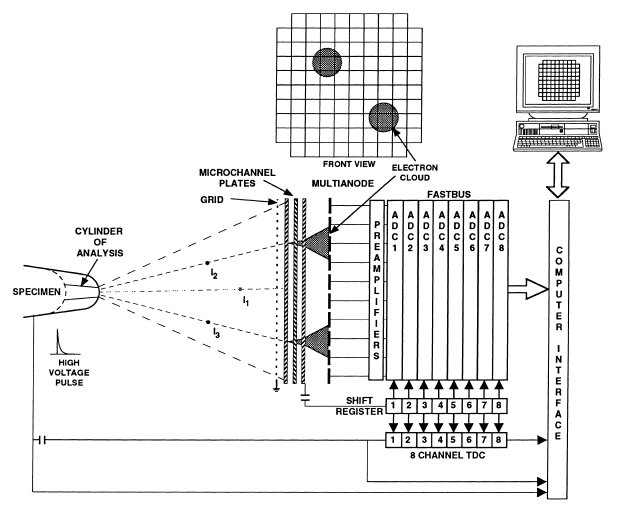
\includegraphics[width=\textwidth]{POSAP}
	}
	\caption{Схема установки POSAP \cite{Deconihout93} Specimen – образец, Microchannel plates – микроканальные пластины, Grid - сетка, Multianode - мультианод, ADC – АЦП(аналого-цифровой преобразователь), High Voltage pulse – импульс высокого напряжения, Channel TDC - канал счета времени, Computer interface – интерфейс подключения к компьютеру}
	\label{fig:POSAP}
\end{figure}

Позиционно-чувствительная детектирующая система состояла из следующих элементов: сетка нулевого потенциала, сборка из МКП, система из 10 анодов и CCD камеры. По сравнению с современными детектирующими системами, данная система отличалась низким быстродействием из-за использования CCD камеры, а также низкой способностью разделять мультисобытия, из-за малого быстродействия. Импульсное напряжение  подавалось напрямую на образец вместе с постоянной его составляющей. На данной установке было получено разрешение по массе на полувысоте ~ 300. Скорость сбора данных составляла примерно 2 иона/секунду. Площадь поперечного сечения исследуемого объема данных составляла примерно 5 × 5  нм.

Одной из первых широко распространенных и успешно используемых установок был так называемый ECOTAP – томографический атомный зонд с компенсацией энергий и оптической системой детектирования (Energy compensated optical tomographic atom probe). Его представила научному сообществу в 1998 году группа под руководством Cerezo в Оксфорде \cite{Cerezo98}. В данной установке используется импульсный высоковольтный способ испарения. Основным преимуществом этого прибора являлась реализация системы компенсации разбросов энергий ионов (рефлектрона). Как было сказано ранее, одним из основных факторов, влияющих на разрешение по массе при импульсном полевом испарении, является разброс энергий ионов, возникающий из-за статистического разброса момента испарения ионов. Соответственно, для решения этой проблемы группа Cerezo установила систему компенсации энергий типа «рефлектрон» , известную в методе времяпролетной масс-спектрометрии. Импульсная добавка напряжения для осуществления контролируемого испарения подавалась на образец с помощью контр-электрода. Контр-электрод – кольцо, расположенное напротив образца на расстоянии примерно 4 мм.

\begin{figure}[htb]
	\centerfloat{
		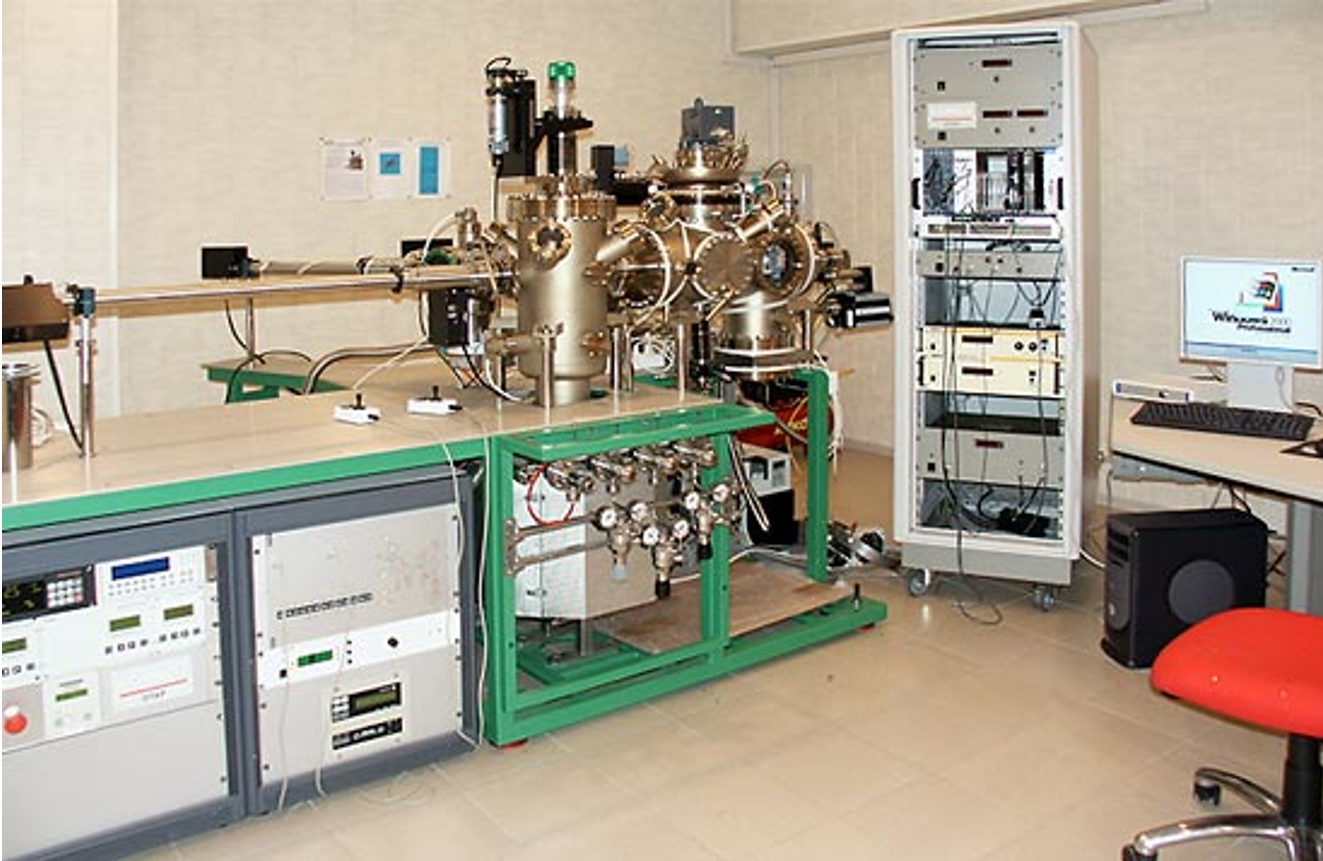
\includegraphics[width=\textwidth]{ECOTAP}
	}
	\caption{Внешний вид установки атомно-зондовой томографии CAMECA ECOTAP}
	\label{fig:ECOTAP}
\end{figure}
Данная установка позволяла получать данные следующего качества:
\begin{itemize}[beginpenalty=10000] % https://tex.stackexchange.com/a/476052/104425
	\item разрешение по массе на 50 \% высоты  $\sim$ 500;
	\item разрешение по массе на 10 \% высоты $\sim$ 250;
	\item угол сбора данных 4-12 град;
	\item сечение объема данных 20 × 20 нм.  
\end{itemize}

	
Помимо реализации рефлектрона, данная установка имела стандартные для того времени технические характеристики:
\begin{itemize}[beginpenalty=10000] % https://tex.stackexchange.com/a/476052/104425
	\item температура образцов 40-80 К;
	\item вакуум < 1 × 10$^{-9}$ Торр; 
	\item частота испаряющих импульсов 2 кГц;
	\item позиционно-чувствительный детектор c ССD камерой;
	\item напряжение на образце 20 кВ; 
	\item газо-инжекционная система;
	\item камеры хранения и загрузки образцов.
\end{itemize}


Установка типа ECOTAP производилась промышленно компанией CAMECA. Один из таких приборов был поставлен в ИТЭФ (Россия) в 2002 г. (Рисунок \cref{fig:ECOTAP}), где эксплуатируется по настоящее время \cite{Suvorov06}.

В 2000-2010 годах появилась возможность использовать компактные лазерные системы испарения, обладающие необходимой стабильностью характеристик в течении длительного времени работы. С этого момента стало возможным развивать метод лазерного  испарения в атомно-зондовых томографах. Например, в 2007 году группа под руководством Шмитца в Германии \cite{Stender07} представила установку атомно-зондовой томографии с 2-мя типами испарения (лазерное и высоковольтное импульсное) и с 3-мя различными относительными расположениями образца и детектора (для варьирования длины пролета, угла сбора данных, возможности использовать рефлектрон). На Рисунке \cref{fig:Schmitz} представлена схема расположения детекторов и вакуумных объемов данной установки. 

\begin{figure}[htb]
	\centerfloat{
		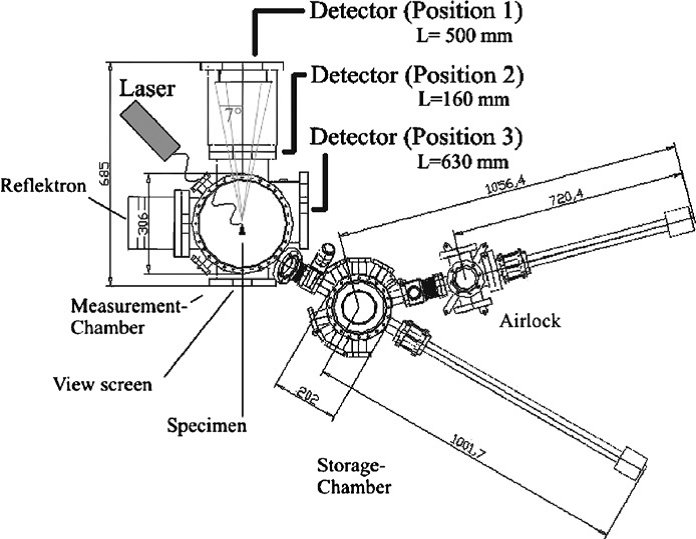
\includegraphics[width=\textwidth]{Schmitz}
	}
	\caption{Схема вакуумных объемов и положения детектирующих систем, вид сверху установки \cite{Stender07}.  Laser - лазер, Specimen - образец, Storage chamber – камера хранения образцов, View screen – смотровое окно, Airlock – камера загрузки, Measurement chamber – анализационный объем,Reflektron - рефлектрон, Detector – детектор. Все размеры на схеме указаны в мм}
	\label{fig:Schmitz}
\end{figure}

Установка, собранная научной группой Шмитца, позволяет использовать как лазерное, так и импульсно-полевое испарение. Лазерный луч находится под острым углом к оси образца. При этом в случае лазерного испарения используется прямопролетная геометрия (положение детектора №1 и №2 на Рисунке \cref{fig:Schmitz}), два различных расстояния от детектора до образца позволяют менять угол сбора данных и длину пролета, что определяет объем собираемых данных и величину разрешения по массе. В случае полевого испарения образец вместе с криосистемой поворачивается в строну рефлектрона, который используется для компенсации энергий ионов при импульсно-полевом испарении. Также, помимо основного вакуумного объема с образцом и детекторами, в состав установки входят загрузочная камера и камера хранения образцов с соответствующими штоками для перемещения образцов. Для поддержания вакуума 1-2×10$^{-10}$ мбар используются турбомолекулярные насосы со скоростями откачки 500/250/70 л/сек. Как уже выше было указанно, в данной установке имеется возможность поворачивать образец на 360 град вокруг вертикальной оси и ± 45 град относительно горизонтальной оси. Охлаждение образца обеспечивается с помощью двух ступенчатой криосистемы Rigon с минимальной температурой 25 К. В ходе проведения исследований различных образцов на данной установке было показано, что она имеет следующие характеристики:
\begin{itemize}[beginpenalty=10000] % https://tex.stackexchange.com/a/476052/104425
	\item угол сбора данных до 39 град;
	\item разрешение по массе 50 \% высоты $\sim$ 300;
	\item сечение объема данных 50 × 50 нм$^{2}$;
	\item среднее количество собранных данных $\sim$5 млн.
\end{itemize}	

В 2002-2003 годах в Америке была представлена первая установка с так называемым локальным электродом LEAP\cref{fig:leap3000}.  Соответственно, наличие локального электрода обуславливало преимущество по качеству данных над большинством остальных установок и определяло дальнейшее интенсивное развитие именно данного семейства установок \cite{Kelly00}. Позднее, в 2006 г. в LEAP появилась возможность устанавливать и лазерную испаряющую систему. В таком случае постоянное напряжение по-прежнему подавалось на локальный электрод, что обеспечивало высокое разрешение по массе и более «мягкие» условия испарения.

Помимо системы испарения, данные установки отличаются наличием улучшенной версией позиционно-чувствительного детектора на основе линий задержки. Вопрос детектирования как можно большего процента испарённых ионов, а также мультисобытий, является одним из ключевых, так как он влияет на чувствительность прибора и на точность определения концентраций. С целью улучшения точности детектирования в установках LEAP используется дополнительный анод уже к двум имеющимся на детекторе. Таким образом, данная детектирующая система позволяет различать наибольшее число мультисобытий из всех существующих ныне позиционно-чувствительных детекторов, применяющихся в АЗТ.
Вакуумная система на LEAP построена по наиболее распространенной схеме. Но если камера проведения анализа или камера хранения по функционалу практически не отличаются от аналогичных установок, то камера загрузки может быть оборудована специальной системой плазменной очистки локальных электродов для продления срока их службы. Вакуум 2×10$^{-10}$ мбар в анализационном объеме обеспечивают как турбомолекулярные насосы, так и ионный насос с титановой присадкой. Все вакуумные объемы приспособлены для отжига до температуры $\sim$ 150 \textdegree С.
Как уже упоминалось, на LEAP может быть установлены как импульсно-полевая, так и лазерная системы испарения. Также существует возможность заказать установку с 2 типами системы испарения. Соответственно, во всех случаях, когда присутствует полевая система испарения, установка дополняется системой компенсации энергий ионов.

Процент детектируемых ионов имеет значение 50 \% для варианта установки с энергокомпенсирующей системой и 80 \% для системы с прямопролетной геометрией. Порог чувствительности к детектированию элементов малых концентраций в анализируемом образце находится на уровне 3-7 ppm (частиц на миллион).
Импульсный источник напряжения может генерировать импульсы с амплитудой до 1400 В. Частота следования импульсов может составлять до 500 кГц. Постоянное напряжение на образце может варьироваться до 15 кВ. Лазерная испаряющая система может работать на частотах вплоть до 2 МГц.
Длительность лазерного импульса - менее 1 пс. Диаметр пучка лазера на образце принимает значения от 3 до 10 мкм, в зависимости от настройки фокусировки. В силу малости диаметра пучка, а также для повышения стабильности условий испарения в процессе эксперимента, программа управления установкой в ходе сбора данных периодически проводит автоматическую проверку наведения пучка.

\begin{figure}[htb]
	\centerfloat{
		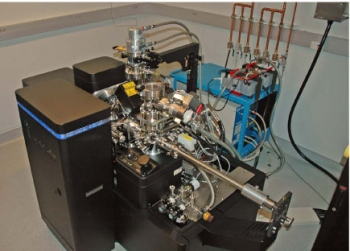
\includegraphics[width=\textwidth]{leap3000}
	}
	\caption{Внешний вид установки атомно-зондовой томографии LEAP 3000X}
	\label{fig:leap3000}
\end{figure}

Получаемое разрешение по массе на установках сильно зависит от исследуемого материала и типа испарения. Как правило, разрешение по массе на полувысоте для лазерного испарения не опускается ниже 1000, но может достигать и значений в 1500. Для вариантов с импульсным высоковольтным  испарением разрешение по массе на полувысоте составляет примерно 400 -1000. Угол сбора данных также сильно зависит от материала и условий исследования, но максимальное заявленное сечение получаемого объема составляет 250~×~250~нм.

В настоящий момент CAMECA предлагает две ключевых конфигурации установки атомно-зондовой томографии LEAP 6000(Invisio 6000) и EIKOS. LEAP позиционируется как наиболее полный и многофункциональный инструмента для широкого круга самых передовых научных задач. Он может быть оснащен лазерным, полевым испарением, а также одновременным испарением с помощью и лазера и импульсного напряжения. Данная установка может быть дополнены криогенной съемной загрузочной камерой (ссылка на криотрансфер), которая позволяет исследовать жидкие объекты в замороженном состоянии \cite{Schwarz20}. Длина волны лазерной системы составляет 257,5 нм. EIKOS  позиционируется как простая и менее требовательная к квалификации персонала и к пробоподготовке установка. Одним из основных её применений производитель видит - промышленность. Ниже на Рисунках \cref{fig:EIKOS,fig:LEAP6000} представлен внешний вид EIKOS и LEAP 6000 соответственно.

\begin{figure}[htb]
	\centerfloat{
		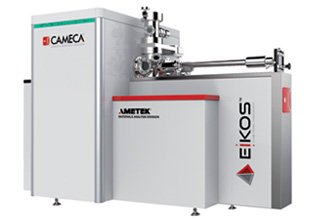
\includegraphics[width=\textwidth]{EIKOS}
	}
	\caption{Внешний вид установки атомно-зондовой томографии EIKOS}
	\label{fig:EIKOS}
\end{figure}

\begin{figure}[htb]
	\centerfloat{
		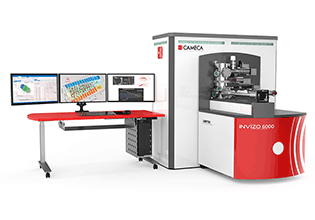
\includegraphics[width=\textwidth]{LEAP6000}
	}
	\caption{Внешний вид установки атомно-зондовой томографии LEAP 6000}
	\label{fig:LEAP6000}
\end{figure}

\FloatBarrier

Среди современных установок также стоит отметить попытки создания комплексных устройств, включающих в себя комбинацию атомно-зондового томографа и другой аналитической установки или методики. В качестве второй установки может выступать СЭМ с ФИП, как в концепции группы Stender \cite{Stender22} или сканирующий туннельный микроскоп, как в концепции группы Umemura \cite{Umemura19}. Также для ряда задач, например для изучения динамики каталитических процессов, атомно-зондовые томографы могут оснащаться дополнительным оборудованием, например газовыми реакторами \cite{Lambeets20}.

\section{Влияние условий испарения на АЗТ данные}\label{sec:ch1/sec5} 

Контролируемое лазерное испарение атомов в АЗТ возможно благодаря нескольким факторам, в том числе: высокое электростатическое поле на образце, периодическое воздействие лазерного излучения, форма образца, низкая температура образца и вероятностный характер процесса десорбции и ионизации атомов. Каждый из приведенных факторов может влиять на качество получаемых АЗТ данных. При этом после сбора и обработки данных важно получить корректные и наиболее достоверные результаты АЗТ исследования. Соответственно, необходимо изучать зависимость качества данных от условий исследования. Далее будут рассмотрены основные используемые подходы к получению характерных зависимостей качества АЗТ данных от параметров и условий испарения.

Исходя из описанных в разделе \cref{sec:ch1/sec1} выражений для вероятности испарения и для высоты энергетического барьера для десорбции и ионизации атома (см. формулы  \cref{eq:equation5,eq:equation6}) можно сделать, что температура образца, приложенное электрическое поле и свойства материала образца являются основными факторами, влияющими на процесс испарения.

Для описания способности материала к более или менее интенсивному используется понятие поле испарения \cite{Vurpillot16} (см. формула \cref{eq:equation5}). Очевидно, что в случае многокомпонентного материала с наноразмерными особенностями (кластеры или фазы) поле испарения для образца в целом будет являть собой некоторую комбинацию локальных полей испарения для матрицы и частицы, и полей испарения для каждого элемента состава материала. Поэтому сложно оценить численно необходимое поле для испарения. Обычно в этом случае исследователям необходимо провести предварительные калибровочные исследования. В процессе такой работы проводится сбор АЗТ данных при различных параметрах испарения, с последующим определением наиболее оптимальных. 

Как выше было сказано, условия испарения можно менять, варьируя некоторые параметры исследования, например, температуру образца и мощность лазерного излучения (в случае использования лазерного испарения). В работе группы Tu \cite{Tu15} приведен достаточно информативный и подробный пример подбора параметров исследования модельного сплава Ni-Al-Mo. Изучены зависимости концентрации элементов от мощности лазера и температуры образца.  Все исследования проведены при постоянной скорости испарения. В случае повышения мощности лазерного излучения наблюдается большее разрешение по массе. Это можно объяснить тем, что в случае низкой мощности лазера, из-за медленного остывания иголки после нагрева лазерным излучением, вероятность испарения атома сохраняется большой на большем промежутке времени, чем при высокой мощности лазера. К негативным эффектам большой мощности можно отнести большую вероятность появления молекулярных ионов и гидридов (подробное объяснение можно найти в \cite{GaultBOOK}). На Рисунке \cref{fig:ParamsComposition} показан пример сравнения масс-спектров при различных условиях испарения.

\begin{figure}[htb]
	\centerfloat{
		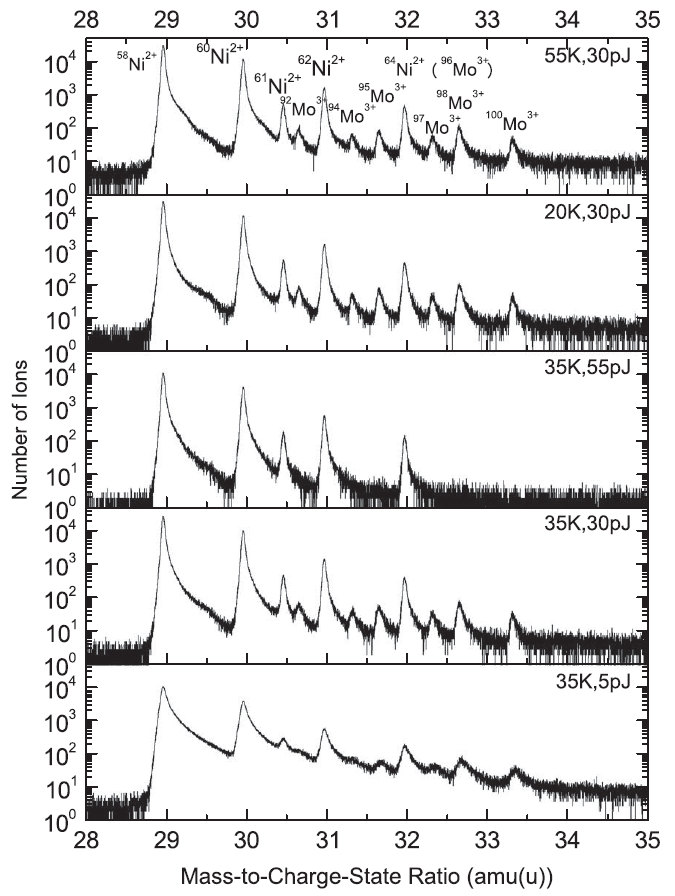
\includegraphics[width=.8\textwidth]{ParamsPower}
	}
	\caption{Сравнение масс-спектров при различной мощности лазера и температуре образца сплава Ni-Al-Mo \cite{Tu15}}
	\label{fig:ParamsPower}
\end{figure}

Также в работе Tu \cite{Tu15} показано, что изменение базовой температуры образца приводит изменению соотношения зарядностей элементов при изменении мощности лазерного излучения, что будет важно к контексте обсуждения способов контроля условий испарения. При этом базовая температура образца практически не вносит искажений в измеряемые концентрации элементов.

Стоит отметить, что слишком высокая мощность лазерного излучения может приводить к ухудшению точности восстановления 3D координат. В работе \cite{Cerezo07} показано, что при избыточной мощности лазера происходит падение пространственного разрешения вследствие перегрева образца (см. Рисунок \cref{fig:ParamsEnergy}).

\begin{figure}[htb]
	\centerfloat{
		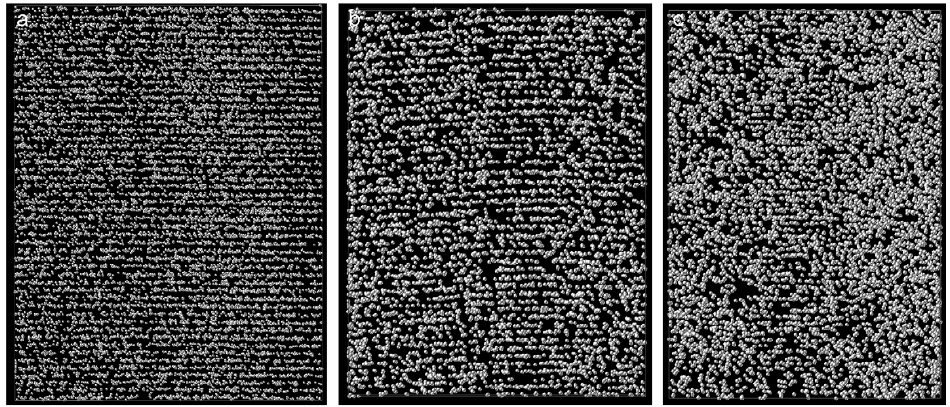
\includegraphics[width=\textwidth]{ParamsEnergy}
	}
	\caption{Срез 3D изображений образца из W, полученных при трех энергиях импульса лазера – 0.4, 1.6 и 2.0 нДж, соответственно \cite{Cerezo07}}
	\label{fig:ParamsEnergy}
\end{figure}

Но выше было сказано, поле испарение может изменяться также с помощью температуры. А точнее в лазерном испарении важнейшую роль при получения более качественных данных играет скорость охлаждения образца и эффективность адсорбции энергии лазера образцом. В работе группы Vella \cite{Vella18} для кремниевого образца с помощью моделирования показана зависимость плотности адсорбируемой энергии в зависимости от расстояния от кончика образца для двух разных углов раствора АЗТ иголки. Расчеты проводились в том числе для двух образцов с разными углами раствора.

\begin{figure}[htb]
	\begin{minipage}[b]{0.49\textwidth}\centering
		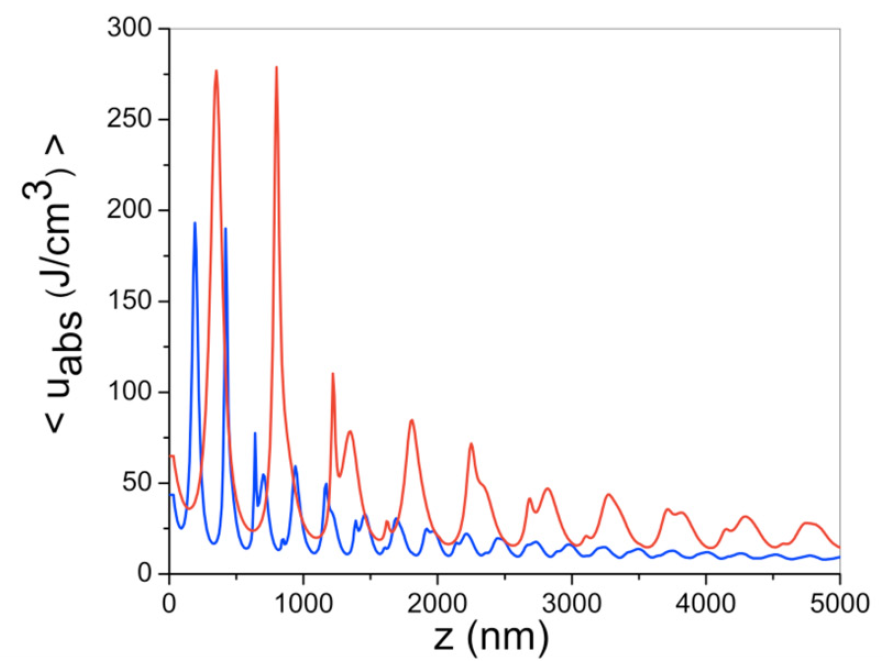
\includegraphics[width=\textwidth]{VellaIntensities} \\ а)
	\end{minipage}
	\begin{minipage}[b]{0.49\textwidth}\centering
		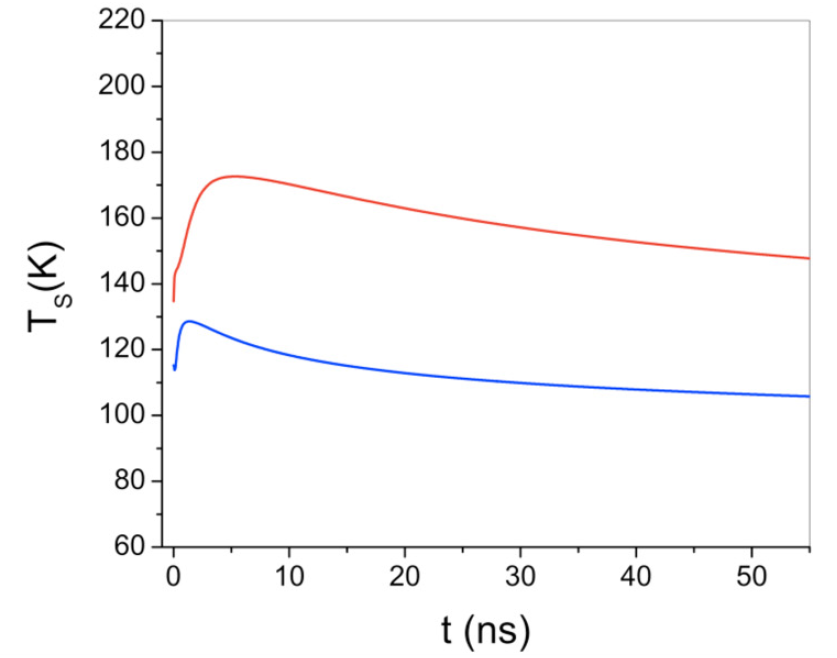
\includegraphics[width=\textwidth]{VellaTemperature} \\ б)
	\end{minipage}
	\caption{а) - Зависимость плотности адсорбированной энергии от расстояния до кончика образца для двух иголок с разным раствором угла. Красная линия - 6\textdegree, синяя - 13.6\textdegree. б) - Зависимость температуры поверхности образца от времени для тех же двух иголок \cite{Vella18}}
	\label{fig:VellaIntensities}
\end{figure}


На Рисунке \cref{fig:VellaIntensities} видно два основных момента, которые играют важную роль в скорости охлаждения образца. Во-первых максимум интенсивности отстоит от кончика образца на некоторое расстояние, соответственно для более тонкого образца (красная линия) тепло "дойдет" до кончика медленнее, чем для образца большей конусности (синяя линия). Во-вторых максимумы для более "тонкого" образца (красная линия) имеют большую интенсивность. Оба этих фактора приводят к тому, что образец с меньшим углом раствора (синий) будет медленнее нагреваться и дольше остывать, что приведет к ухудшению масс-спектра. Данный эффект наглядно показан на Рисунке \cref{fig:VellaSpectors}.

\begin{figure}[htb]
	\centerfloat{
		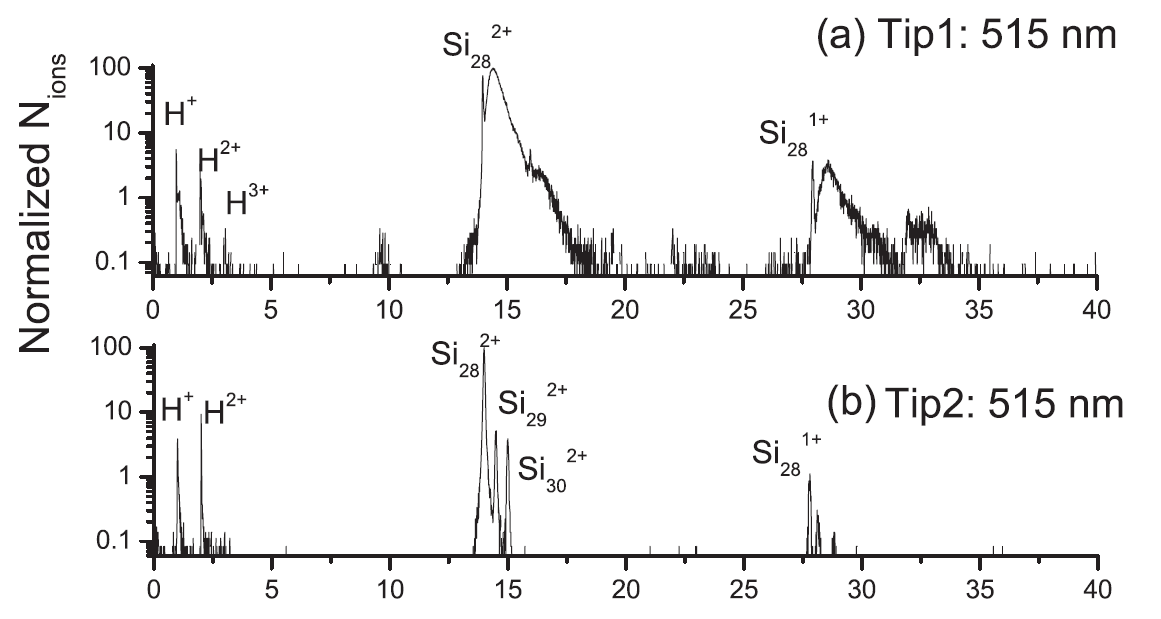
\includegraphics[width=\textwidth]{VellaSpectors}
	}
	\caption{Сравнение масс-спектров при различном угле раствора образца из кремния (a) - образец с углом раствора 6\textdegree, (b) - 13.6\textdegree \cite{Vella18}}
	\label{fig:VellaSpectors}
\end{figure}

Также стоит отметить, что на качество масс-спектра влияют: скорость испарения \cite{Raznitsyn18}, длина волны лазерного излучения и радиус закругления кончика образца \cite{Houard10} и некоторые другие факторы(частота лазера, ионно-фокусирующие системы, конструкция держателя образцов, локальный электрод, диаметр пучка лазерного излучения и т.д.). При этом в процессе исследования может изменяться состав исследуемого материала, например, при испарении разных фаз или многослойных материалов. Большое число параметров исследования, влияющих на получаемые данные делает задачу контроля условия испарения сложной и уникальной для каждой из конструкцию атомно-зондовых установок, а зачастую и для каждого исследуемого материала. 

Для оценки качества данных АЗТ исследователи зачастую пользуются двумя или тремя метриками. При этом есть ряд характеристик данных, которые могут редко указываться в печати. Какого-либо общего подхода к сравнению  и оценке качества атомно-зондовых данных не приведено. Наиболее распространенная оценка <<хороших>> или <<плохих>> условия испарения это то, получена ли ожидаемая концентрация химических элементов и разрешение по массе. Например, в вышеупомянутой работе группы Tu \cite{Tu15} приводятся графики зависимостей концентрации от мощности лазерного излучения и от температуры образца (Рисунок \cref{fig:TuComposition}). Получение таких зависимостей является наиболее часто встречающейся методикой подбора параметров исследования. 

\begin{figure}[htb]
	\begin{minipage}[b]{0.49\textwidth}\centering
		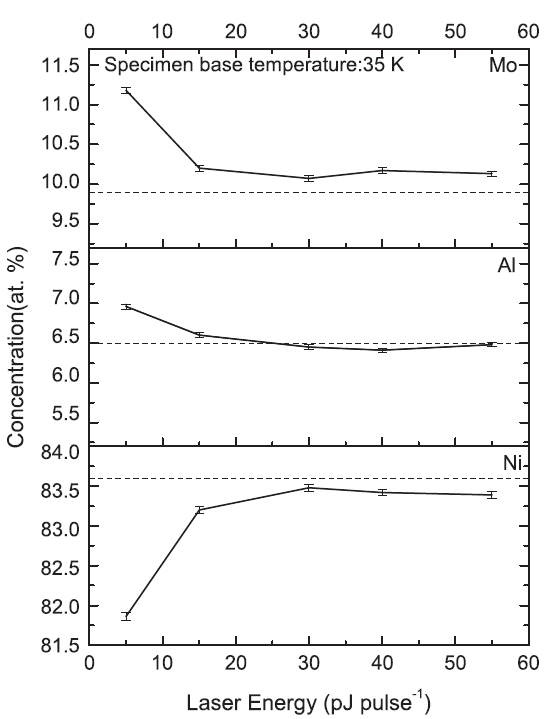
\includegraphics[width=\textwidth]{TuPower} \\ а)
	\end{minipage}
	\begin{minipage}[b]{0.49\textwidth}\centering
		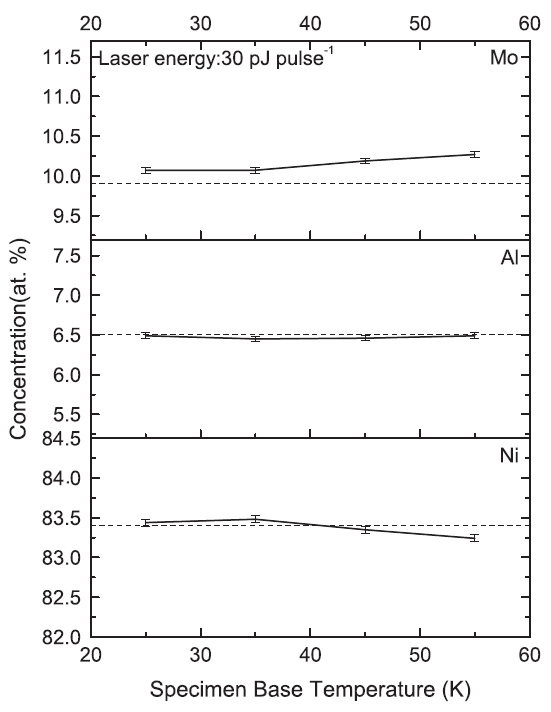
\includegraphics[width=\textwidth]{TuTemperature} \\ б)
	\end{minipage}
	\caption{а) Зависимость концентрации от мощности лазерного излучения. б) Зависимость концентраций от базовой температуры образца \cite{Tu15}}
	\label{fig:TuComposition}
\end{figure}

Как видно, отклонение детектируемых концентраций элементов от истинных значений велико при малой энергии импульса, и уменьшается при ее возрастании. Для приведенных данных оптимальная мощность для оценки концентраций выбрана примерно в середине диапазона мощности лазерной системы, где ошибка одновременно по трем элементам сплава наименьшая. Однако утверждается, что с возрастанием мощности лазера разница в полях испарения элементов, составляющих материал, уменьшается, что благоприятно сказывается на точности определения концентрации. Но, как уже было отмечено, мощность ограничена сверху эффектами поверхностной миграции, а также нарушениями в составе испаряемых элементов (например, за счет испарения молекулярных ионов, таких как ионы $Mo^{+2}$) \cite{Tu15}. Поэтому энергия импульса, с целью улучшения разрешения по массе и точности определения концентраций, должна выбираться максимально возможной в пределах, ограниченных эффектами перегрева образца \cite{Tu15}. Также следует отметить, что, в случае исследования диэлектрических включений в металлах, для достижения точного стехиометрического состава, необходимо несколько снижать энергию импульса, по сравнению со случаем исследования металла без таких включений \cite{LarsonBOOK}.


Важно отметить, что напрямую контролировать концентрации элементов в материале довольно сложно, так как перед получение точных значений концентраций необходимо провести многоэтапную обработку данных. Эту обработку практически невозможно проводить <<налету>>, во время исследования. Соответственно, необходимо выбрать другие метрики или искать косвенные зависимости качества данных от параметров исследования. Также стоит отметить, что для повторяемости результатов важно оперировать теми параметрами и характеристиками, которые могут быть рассчитаны независимо от конструкции и типа установки (единственное ограничение - желательно сравнивать исследования при фиксированном типе испарения).

В свою очередь разрешение по массе очень легко рассчитывать, поскольку вне зависимости от качества обработки данных - всегда можно оценить ширину тех или иных пиков на масс-спектре. Очень часто в работах данная метрика используется как абстрактный показатель качества данных при сравнении установок \cite{Tegg23}. При этом данная метрика может не учитывать значения концентраций или качество 3D восстановления координат.

В последних исследованиях наиболее удобным выбором метрики для сравнения условий испарений видится соотношение зарядностей для одного или для нескольких элементов \cite{Tu15,Vurpillot16,Diercks13,Mancini14}. В некоторых источниках данную метрику можно увидеть под аббревиатурой CSR (charge state ratio - соотношение зарядностей), вычисляется как отношение $E^{n+}/E^{m+}$, где Е - химический элемент, n и m - величины заряда ионов. К преимуществам CSR можно отнести следующие особенности:
\begin{itemize}
	\item CSR связан с поверхностным полем образца. Эту связь была впервые оценена в работе Kingham \cite{Kingham82}.
	\item В рамках одного исследования можно легко оценить тенденции изменения состава образца и/или формы его кончика.
	\item Можно проводить сравнение условий испарения для разных образцов одного материала, что довольно сложно, поскольку необходимо учитывать напряженность поля, энергию лазерного импульса или величину импульса напряжения.
	\item CSR можно рассчитывать как для всего образца, так локально для небольшой области образца (например, вокселя), что позволяет в ряде случаев устанавливать взаимосвязи между локальным полем и локальным изменением состава.
	\item Соотношение зарядностей позволяет сравнивать исследования, проведенные на разных установках и разными пользователями.
\end{itemize} 

Помимо соотношения зарядностей в исследованиях могут использовать другие параметры для оценки качества данных. Один из наиболее важных параметров - доля мультисобытий \cite{Valderrama15}. Число мультисобытий опосредованно дает возможность оценить качество испарения. Формально, чем больше доля мультисобытий - тем менее оптимальны условия испарения. К минусам такой метрики можно отнести высокую зависимость от качества восстановления данных на детектирующей системе \cite{DaCosta12}.

В качестве дополнительных метрик оценки качества данных могут использоваться следующие характеристики: количество шума в определенном промежутке масс-спектра \cite{Valderrama15}, точность 3D восстановления \cite{Tegg23}, скорость испарения \cite{Raznitsyn18}.


\FloatBarrier

\section{Заключение к главе 1}\label{sec:ch1/sec6}

В главе были изложены основные теоретические основы метода атомно-зондовой томографии. Описана общая схема проведения эксперимента и подробно описаны узлы типичной установки атомно-зондовой томографии. Показана важность выбора условий проведения исследований, в том числе описаны основные используемые метрики качества АЗТ данных. Сведения, описанные в рамках данной главы легли в основу нового атомно-зондового томографа ПАЗЛ-3D, конструкция и принцип работы которого описывается далее.



























